% ====================================================================
%+
% SECTION NAME:
%    \secname.tex
%
% CHAPTER:
%    cosmology.tex
%
% ELEVATOR PITCH:
%    Lensed quasars and supernovae provide distance measurements for
%    cosmology. They are a few days to a few weeks in length. To
%    measure them well we need long campaigns (>~3 years) with high
%    night-to-night cadence (better than the standard 5 days if
%    possible, especially as combining all filters might be difficult.)
%
% COMMENTS:
%
%
% BUGS:
%
%
% AUTHORS:
%   Phil Marshall (@drphilmarshall)
%-
% ====================================================================
\clearpage
\section{ Strong Gravitational Lens Time Delays }
\def\secname{lenstimedelays}\label{sec:\secname}

\credit{drphilmarshall},
\credit{rhiannonlynne}

% This individual section will need to describe the particular
% discoveries and measurements that are being targeted in this section's
% science case. It will be helpful to think of a ``science case" as a
% ``science project" that the authors {\it actually plan to do}. Then,
% the sections can follow the tried and tested format of an observing
% proposal: a brief description of the investigation, with references,
% followed by a technical feasibility piece. This latter part will need
% to be quantified using the MAF framework, via a set of metrics that
% need to be computed for any given observing strategy to quantify its
% impact on the described science case. Ideally, these metrics would be
% combined in a well-motivated figure of merit. The section can conclude
% with a discussion of any risks that have been identified, and how
% these could be mitigated.

% A short preamble goes here. What's the context for this science
% project? Where does it fit in the big picture?

The multiple images of strongly lensed quasars and supernovae have
delayed arrival times: variability in the first image will be observed
in the second image some time later, as the photons take different
paths around the deflector galaxy, and through different depths of
gravitational potential. If the lens mass distribution can be modeled
independently, using a combination of high resolution imaging of the
distorted quasar/SN host galaxy and stellar dynamics in the lens
galaxy, the measured time delays can be used to infer the``time delay
distance'' in the system. This distance enables a direct measurement
of the Hubble constant, independent of the distance ladder.

% --------------------------------------------------------------------

\subsection{Target measurements and discoveries}
\label{sec:\secname:targets}

% Describe the discoveries and measurements you want to make.

For this cosmological probe to be competitive with LSST's others, the
time delays of several hundred systems (which will be distributed
uniformly over the extragalactic sky) will need to be measured with
bias below the sub-percent level, while the precision required is a
few percent per lens.  In galaxy-scale lenses, the kind that are most
accurately modeled, these time delays are typically between several
days and several weeks long, and so are measurable in monitoring
campaigns having night-to-night cadence of between one and a few days,
and seasons lasting several months or more.

% Now, describe their response to the observing strategy.
% Qualitatively, how will the science project be affected by the
% observing schedule and conditions? In broad terms, how would we
% expect the observing strategy to be optimized for this science?

To obtain accurate as well as precise lensed quasar time delays, several monitoring seasons are required. Lensed supernova time delays have not yet been measured, but their transient nature means that their time delay measurements may be more sensitive to cadence than season or campaign length.

% --------------------------------------------------------------------

\subsection{Metrics}
\label{sec:\secname:metrics}

% Quantifying the response via MAF metrics: definition of the metrics,
% and any derived overall figure of merit.

Anticipating that the time delay accuracy would depend on night-to-night cadence, season length, and campaign length, we carried out a large scale simulation and measurement program that coarsely sampled these schedule properties. In \citet{LiaoEtal2015}, we simulated 5 different light curve datasets, each containing 1000 lenses, and presented them to the strong lensing community in a ``Time Delay Challenge.'' These 5 challenge ``rungs'' differed by their schedule properties, in the ways shown in \autoref{tab:tdcrungs}. Focusing on the best challenge submissions made by the community, we derived a simple power law model for the variation of each of the time delay accuracy, time delay precision, and useable sample fraction, with the schedule properties cadence, season length and campaign length. These models are shown in \autoref{fig:tdcresults}, reproduced from \citet{LiaoEtal2015}, and are given by the following equations:
\begin{align}
|A|_{\rm model} &\approx 0.06\% \left(\frac{\rm cad} {\rm 3 days}  \right)^{0.0}
                          \left(\frac{\rm sea}  {\rm 4 months}\right)^{-1.0}
                          \left(\frac{\rm camp}{\rm 5 years} \right)^{-1.1} \notag \\
  P_{\rm model} &\approx 4.0\% \left(\frac{\rm cad} {\rm 3 days}  \right)^{ 0.7}
                         \left(\frac{\rm sea}  {\rm 4 months}\right)^{-0.3}
                         \left(\frac{\rm camp}{\rm 5 years} \right)^{-0.6} \notag \\
  f_{\rm model} &\approx 30\% \left(\frac{\rm cad} {\rm 3 days}  \right)^{-0.4}
                        \left(\frac{\rm sea}  {\rm 4 months}\right)^{ 0.8}
                        \left(\frac{\rm camp}{\rm 5 years} \right)^{-0.2} \notag
\end{align}

%%%%%%%%%%%%%%%%%%%%%%%%%%%%%%%%%%%%
\begin{table*}
\begin{center}
\capstart
\begin{tabular}{cccccc} \hline\hline
  Rung &  Mean Cadence & Cadence Dispersion & Season   & Campaign & Length   \\
       &  (days)       & (days)             & (months) & (years)  & (epochs) \\ \hline
  0    &    3.0        &   1.0              &   8.0    &    5     & 400      \\
  1    &    3.0        &   1.0              &   4.0    &    10    & 400      \\
  2    &    3.0        &   0.0              &   4.0    &    5     & 200      \\
  3    &    3.0        &   1.0              &   4.0    &    5     & 200      \\
  4    &    6.0        &   1.0              &   4.0    &    10    & 200      \\
\hline\hline
\end{tabular}
\end{center}
\caption{The observing parameters for the five rungs of the Time Delay
Challenge. Reproduced from \citet{LiaoEtal2015}.\label{tab:tdcrungs}}
\end{table*}
%%%%%%%%%%%%%%%%%%%%%%%%%%%%%%%%%%%%

%%%%%%%%%%%%%%%%%%%%%%%%%%%%%%%%%%%
\begin{figure*}[!ht]
  \capstart
  \begin{minipage}[b]{\linewidth}
    \begin{minipage}[b]{0.32\linewidth}
      \centering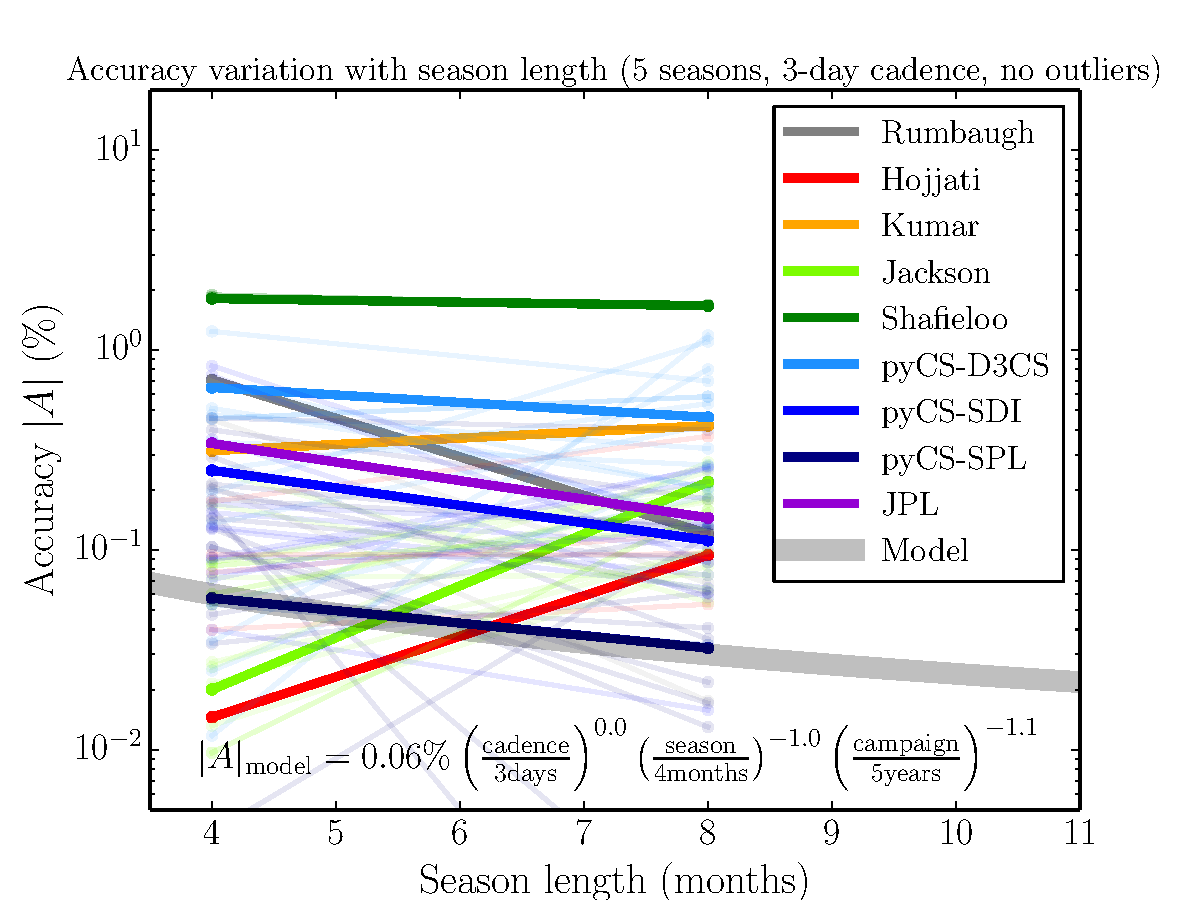
\includegraphics[width=\linewidth]{figs/Accuracy_season_nca.pdf}
    \end{minipage} \hfill
    \begin{minipage}[b]{0.32\linewidth}
      \centering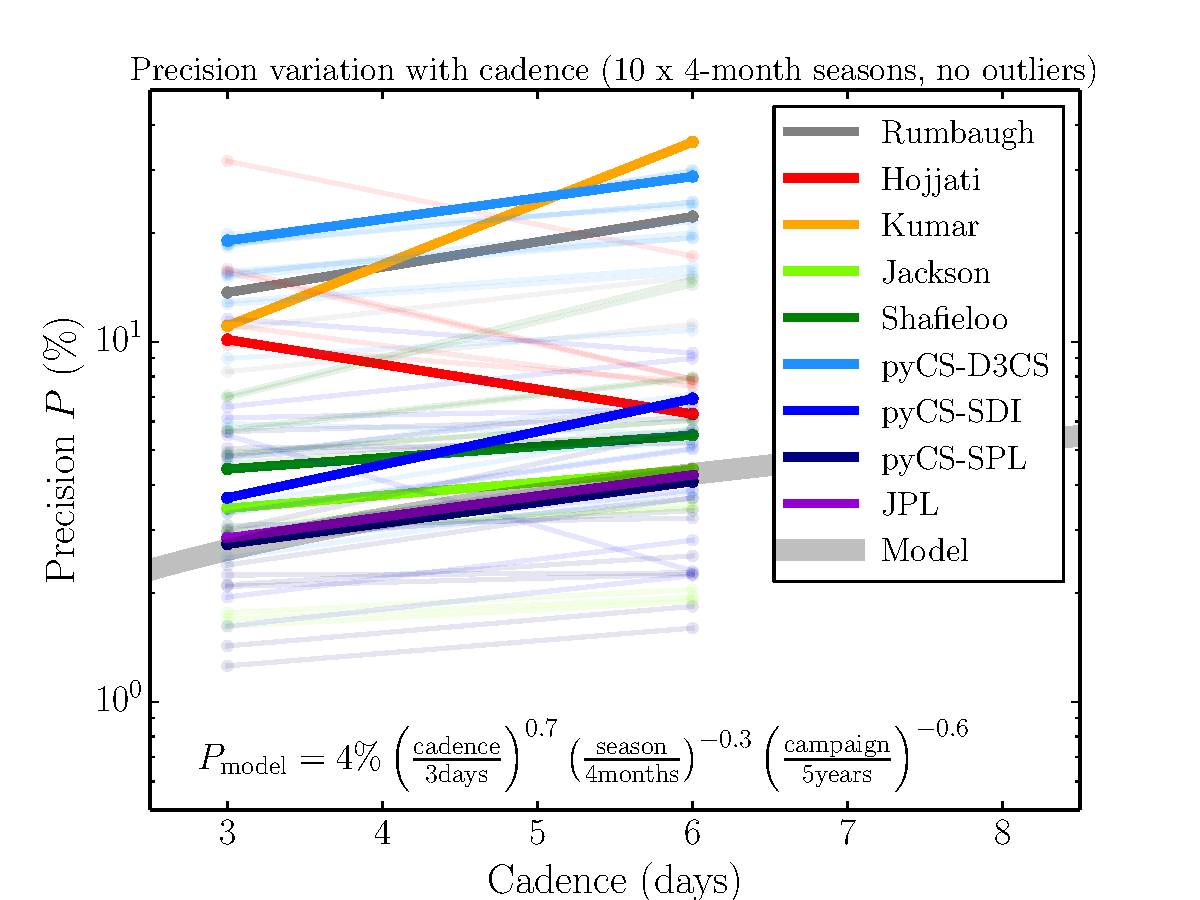
\includegraphics[width=\linewidth]{figs/Precision_cadence_nca.pdf}
    \end{minipage} \hfill
    \begin{minipage}[b]{0.32\linewidth}
      \centering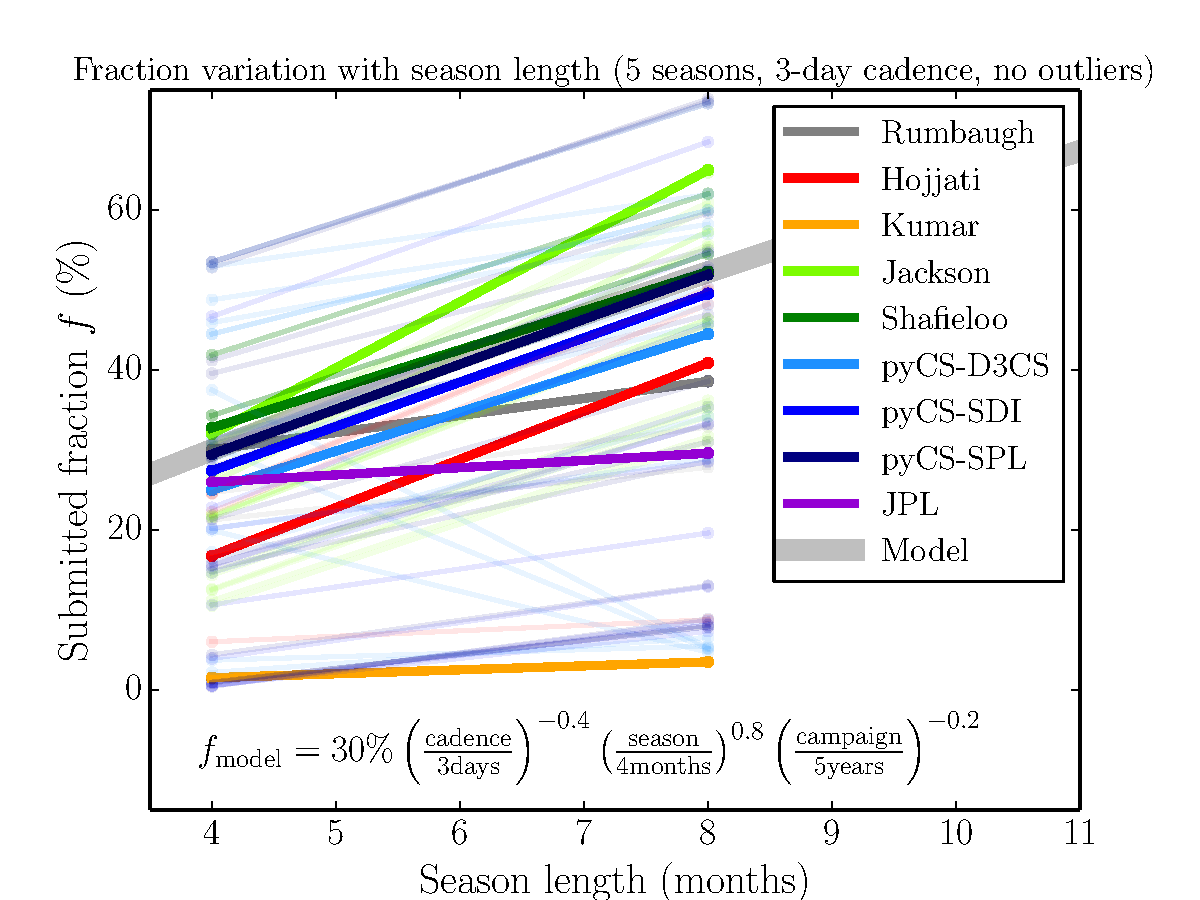
\includegraphics[width=\linewidth]{figs/Fraction_season_nca.pdf}
    \end{minipage}
  \end{minipage}
\caption{Examples of changes in accuracy $A$ (left), precision $P$ (center) and success fraction $f$ (right) with schedule properties, as seen in the different TDC submissions. The gray
approximate power law model was derived by visual inspection of the
pyCS-SPL results; the signs of the indices were pre-determined according to our expectations. Reproduced from \citet{LiaoEtal2015}.}
\label{fig:tdcresults}
\end{figure*}
%%%%%%%%%%%%%%%%%%%%%%%%%%%%%%%%%%%

All three of these metrics would, in an ideal world, be optimized:
this could be achieved by decreasing the night-to-night cadence (to
better sample the light curves), extending the observing season length
(to maximize the chances of capturing a strong variation and its
echo), and extending the campaign length (to increase the number of
effective time delay measurements). A combined figure of merit should
therefore be readily available. The quantity of greatest scientific
interest is the {\it accuracy in cosmological parameters}: efforts to derive
such a figure of merit in terms of the Hubble constant are underway.

% --------------------------------------------------------------------

\subsection{OpSim Analysis}
\label{sec:\secname:analysis}

% OpSim analysis: how good would the default observing strategy be, at
% the time of writing for this science project?

In this section we present the results of our ongoing \OpSim / MAF
analysis, as we try to
answer the question ``how good would the proposed observing
strategies be, for time delay lens cosmography?''

We used the
\simsMAFcontrib{SeasonStacker}{mafContrib/seasonStacker.py} to work
with seasons.

We used \texttt{ops2\_1075} for most of our tests, but we need to now
re-run on \opsimdbref{db:enigma}, and others from \autoref{chp:cadence2015}.

\todo{PJM}{Correct the above paragraphs and add more links to MAF code.}

\autoref{fig:lenstimedelays:results} shows the results of our MAF
analysis of one \OpSim database, \texttt{ops2\_1075}, where we have
assumed that all filters were able to be used in the light curve
analysis (as was implicitly assumed when applying the results of
\citeauthor{LiaoEtal2015}). These sky maps show that, over the main
(WDF) survey area, the time delay accuracy, time delay precision and
time delay lens success fraction are consistently maintained,
indicating that the global average values of these metrics could
conceivably used as higher level metrics or even figure of merit.

\autoref{tab:lenstimedelays:results} shows the global (i.e. al-sky)
average values of our metrics, for two different \OpSim
databases and two different filter set assumptions.

\todo{PJM}{Compute global average lens time delay metrics and discuss.}

%%%%%%%%%%%%%%%%%%%%%%%%%%%%%%%%%%%
\begin{figure*}[!ht]
  \capstart
  \begin{minipage}[b]{\linewidth}
    \begin{minipage}[b]{0.32\linewidth}
      \centering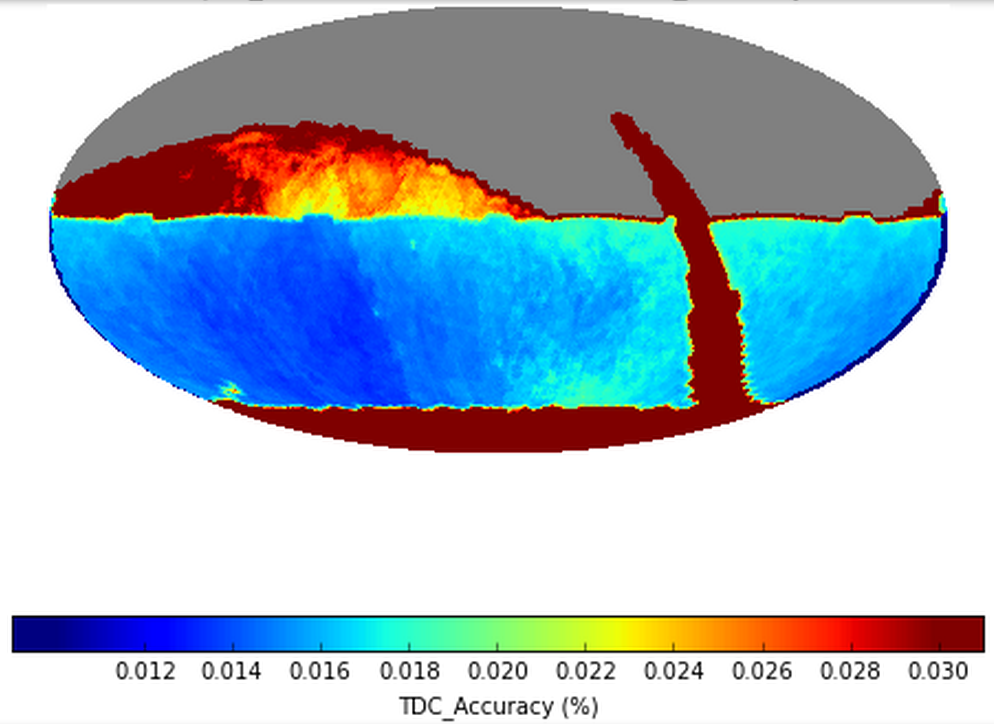
\includegraphics[width=\linewidth]{figs/lenstimedelays-ops2_1075-Accuracy-skymap.png}
    \end{minipage} \hfill
    \begin{minipage}[b]{0.32\linewidth}
      \centering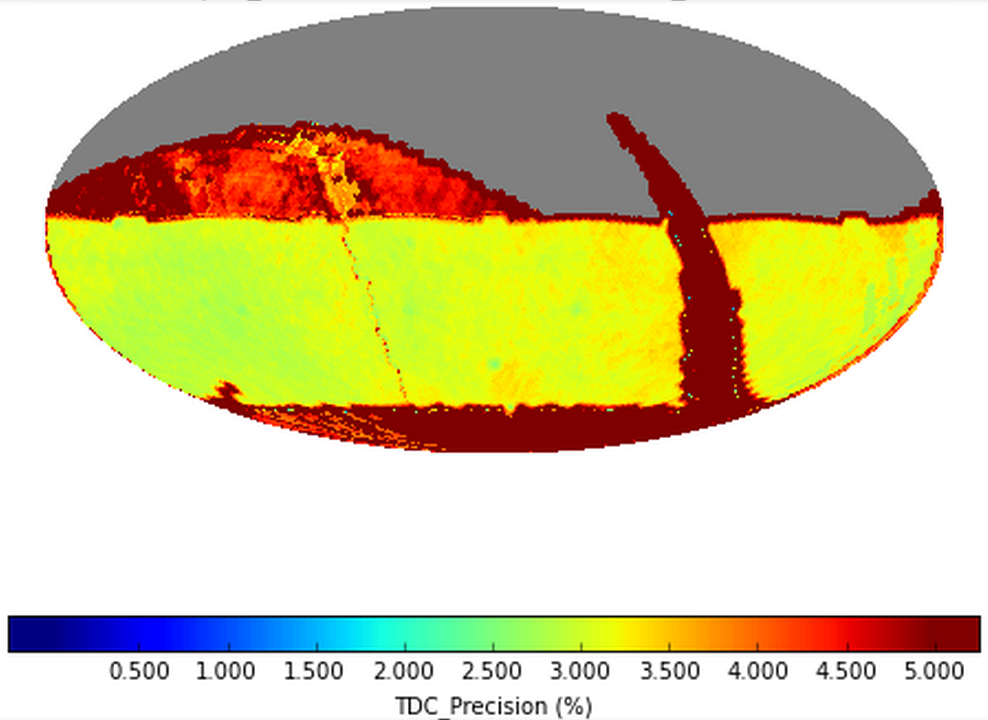
\includegraphics[width=\linewidth]{figs/lenstimedelays-ops2_1075-Precision-skymap.png}
    \end{minipage} \hfill
    \begin{minipage}[b]{0.32\linewidth}
      \centering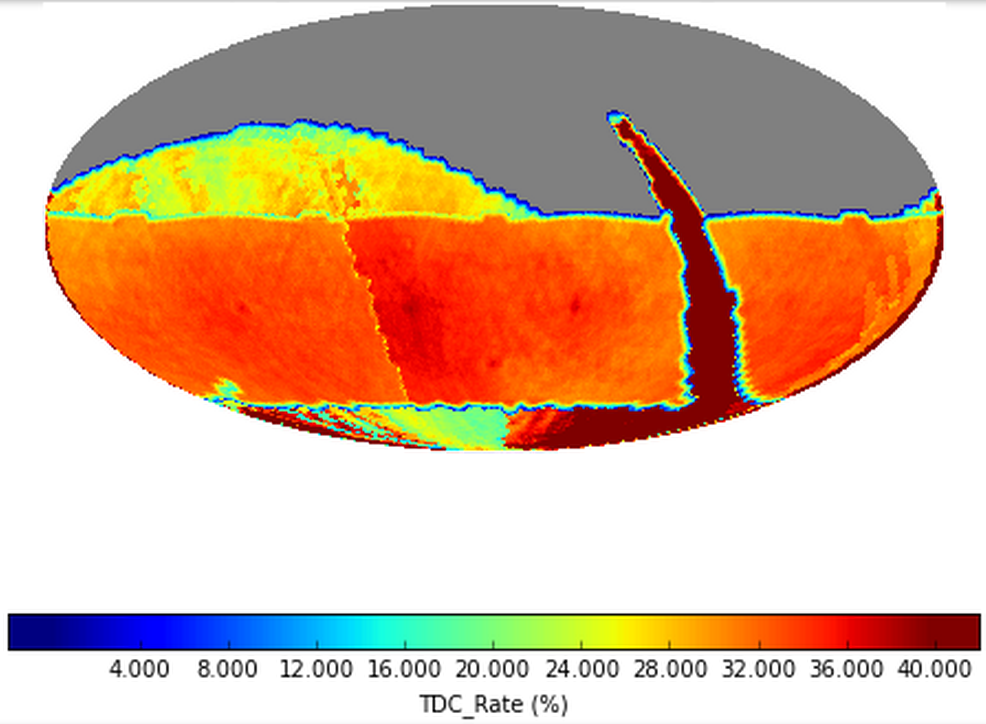
\includegraphics[width=\linewidth]{figs/lenstimedelays-ops2_1075-Fraction-skymap.png}
    \end{minipage}
  \end{minipage}
\caption{Sky maps of the accuracy $A$ (left), precision $P$ (center) and
success fraction $f$ (right) metrics, for the \texttt{ops2\_1075} \OpSim
database and assuming all filters ($ugrizy$) are used in the analysis
according to the assumptions described in the text.}
\label{fig:lenstimedelays:results}
\end{figure*}
%%%%%%%%%%%%%%%%%%%%%%%%%%%%%%%%%%%


%%%%%%%%%%%%%%%%%%%%%%%%%%
\begin{table*}
\begin{center}
\caption{Lens Time Delay Metric Analysis Results.}
\label{tab:lenstimedelays:results}
\footnotesize
\begin{tabularx}{\linewidth}{ccccccccc}
  \hline
  \OpSim run
   & Filters
    & \texttt{cadence}
     & \texttt{season}
      & \texttt{campaign}
       & \texttt{Accuracy}
        & \texttt{Precision}
         & \texttt{Fraction}
          & \texttt{timedelayFoM} \\
  \hline\hline

  \texttt{enigma\_1189}
   & $ri$
    & $XXX$
     & $XXX$
      & $XXX$
       & $XXX$
        & $XXX$
         & $XXX$
          & ??? \\

  \texttt{enigma\_1189}
   & $ugrizy$
    & $XXX$
     & $XXX$
      & $XXX$
       & $XXX$
        & $XXX$
         & $XXX$
          & ??? \\
  \hline

  \texttt{ops2\_1075}
   & $ri$
    & $XXX$
     & $XXX$
      & $XXX$
       & $XXX$
        & $XXX$
         & $XXX$
          & ??? \\

  \texttt{ops2\_1075}
   & $ugrizy$
    & $XXX$
     & $XXX$
      & $XXX$
       & $XXX$
        & $XXX$
         & $XXX$
          & ??? \\
  \hline

\multicolumn{9}{p{\linewidth}}{\scriptsize Notes: see the text for
the definitions of each metric, and sky maps and histogram
plots of them. The Figure of Merit is still under development.}
\end{tabularx}
\normalsize
\medskip\\
\end{center}
\end{table*}
%%%%%%%%%%%%%%%%%%%%%%%%%%


% --------------------------------------------------------------------

\subsection{Discussion}
\label{sec:\secname:discussion}

Discussion: what risks have been identified? What suggestions could be
made to improve this science project's figure of merit, and mitigate
the identified risks?

\todo{PJM}{Write lens time delays discussion section.}


\navigationbar

% ====================================================================
